\chapter{Bonds, antibonds and bond order}
\label{ch:t-bond-order}
\index{Bond order}
\index{Antibonding orbital}
\index{Hydrogen molecule}\index{Helium dimer}
\eccexample{Examples > General Chemistry > Molecular orbitals of diatomics}

Molecular orbital theory explains why two hydrogen atoms form a molecule and two helium atoms do not with one rule: electrons in a bonding orbital hold the atoms together, electrons in an antibonding orbital push them apart, and the bond order is half the difference. This chapter gives the teacher four molecules that make the rule concrete, \chem{H2+}, \chem{H2}, \chem{He2+} and \chem{He2}, with bond orders \textonehalf, 1, \textonehalf{} and 0, and shows a class that the bond order predicts which bonds are shortest and stiffest, and that \chem{He2} has no bond at all.

\section*{This requires}
Nothing beyond ECCE: the calculations are in the General Chemistry example set.

\section{The calculations}
The topic \menu{Molecular orbitals of diatomics} holds \emph{H2\_cation}, \emph{H2}, \emph{He2\_cation} and \emph{He2}. The first three are optimised structures with their vibrational frequencies. \emph{He2} cannot be optimised, because the two atoms do not bind; it is a single calculation with the atoms held \SI{3.0}{\angstrom} apart.

\section{Procedure}
\begin{enumerate}
	\item In the Organizer, choose \menu{File > Open Example Calculations}, pick \menu{General Chemistry} and click \menu{OK}.
	\item Open \emph{H2} in the Viewer and choose \menu{Properties > Orbitals > MOs}. Note which orbitals are occupied and draw the lowest occupied and the lowest empty orbital with \menu{Compute}.
	\item With \menu{Measure} (Chapter~\ref{ch:first-calculation}), measure the H--H distance, and open \menu{Properties > Vibrational spectra > Vibrational Frequencies} for the stretching frequency.
	\item Repeat for \emph{H2\_cation}, \emph{He2\_cation} and \emph{He2} (\emph{He2} has no frequencies).
\end{enumerate}
\index{MOs panel}

\section{Bond order}
Two 1s orbitals combine into two molecular orbitals: $\sigma$, with the electron density gathered between the nuclei, and $\sigma^*$, with a node half way between them. Filling the orbitals from the bottom gives table~\ref{tab:bo}: \chem{H2+} has one electron in $\sigma$, \chem{H2} two, \chem{He2+} two in $\sigma$ and one in $\sigma^*$, and \chem{He2} two in each. The bond order is (bonding electrons $-$ antibonding electrons)/2.

\begin{figure}[htbp]
	\centering
	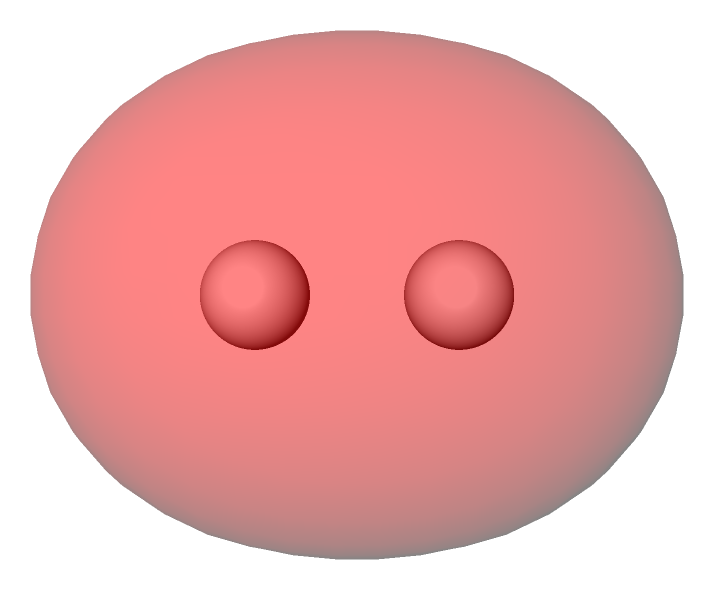
\includegraphics[width=0.3\linewidth]{bond-order/h2-sigma.ecce-9.5.3-dev.png}\hspace{4mm}
	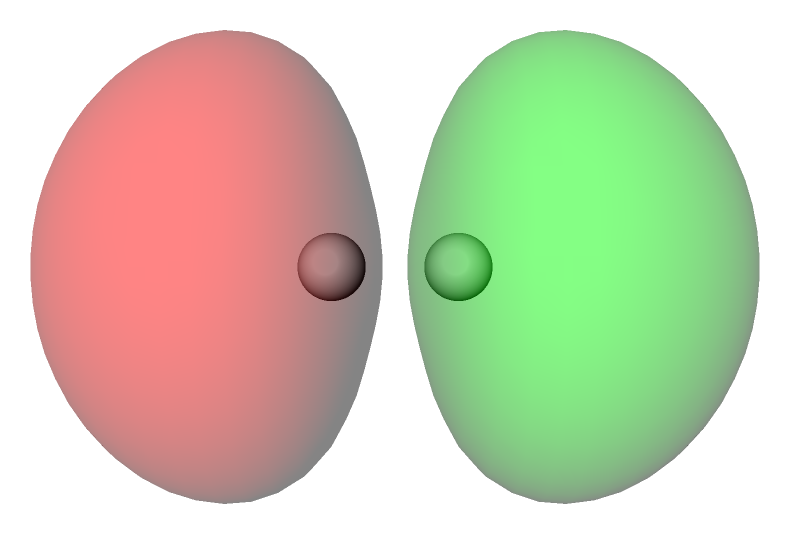
\includegraphics[width=0.3\linewidth]{bond-order/h2-sigmastar.ecce-9.5.3-dev.png}\\[3mm]
	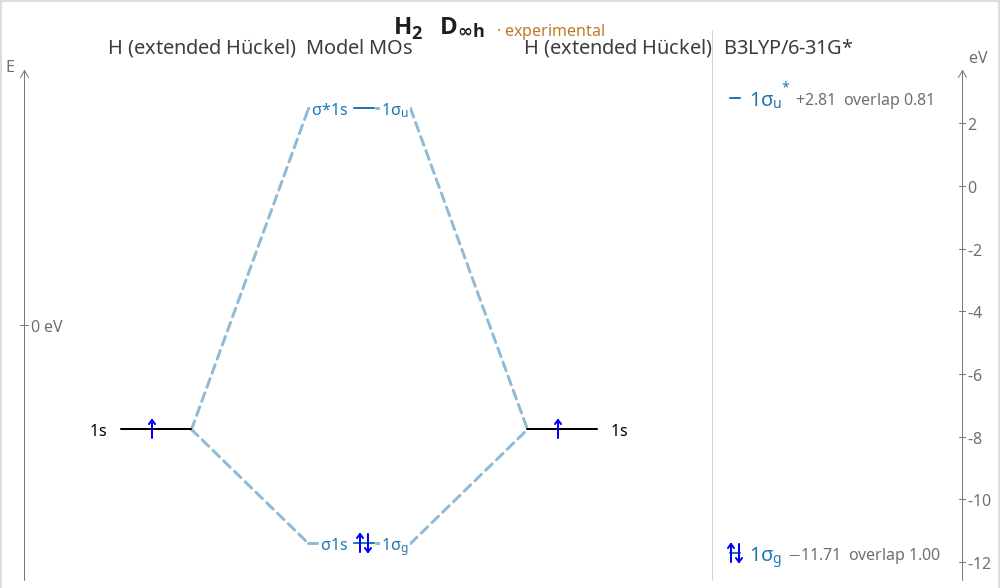
\includegraphics[width=0.75\linewidth]{bond-order/h2-diagram.ecce-9.5.3-dev.png}
	\caption{Top: the bonding $\sigma$ orbital (left) and the empty antibonding $\sigma^*$ orbital (right) of \chem{H2}, drawn in the \menu{MOs} panel; the two colours are the two signs of the orbital. Bottom: the MO diagram of \chem{H2} (\menu{Properties > Orbitals > MO Diagram}): the 1s levels of the two atoms on the left and right, the $\sigma$ and $\sigma^*$ levels between them, and on the far right the levels of the calculation with their energies in eV.}
	\label{fig:bo-h2}
\end{figure}

Figure~\ref{fig:bo-h2} shows that the $\sigma$ orbital is one surface around both nuclei, while $\sigma^*$ is cut in two by an empty plane between them, because in $\sigma$ the two 1s orbitals add and in $\sigma^*$ they cancel half way between the atoms. Hence the electrons in $\sigma$ sit between the nuclei and pull them together, and electrons in $\sigma^*$ sit outside and do not; in the diagram this is the $\sigma$ level below the two 1s levels and the $\sigma^*$ level above them. Each pair of electrons in $\sigma$ is one bond, and each electron in $\sigma^*$ undoes the effect of one in $\sigma$, which is what the bond order counts.

\begin{table}[htbp]
	\centering
	\caption{Electrons in the bonding and antibonding orbitals, bond order, calculated bond length and stretching frequency of the four molecules. The frequency is in wavenumbers (cm$^{-1}$): the higher it is, the stiffer the bond. From the stored ECCE calculations. Measured \cite{nistwebbook}: \chem{H2} \SI{0.741}{\angstrom}; \chem{H2+} \SI{1.052}{\angstrom} and \SI{2322}{cm^{-1}}.}
	\label{tab:bo}
	\begin{tabular}{lccccr}
		\toprule
		Molecule & $\sigma$ & $\sigma^*$ & bond order & bond length (\AA) & frequency (cm$^{-1}$) \\
		\midrule
		\chem{H2}  & 2 & 0 & 1 & 0.743 & 4449 \\
		\chem{H2+} & 1 & 0 & \textonehalf & 1.057 & 2334 \\
		\chem{He2+} & 2 & 1 & \textonehalf & 1.075 & 1746 \\
		\chem{He2} & 2 & 2 & 0 & no bond & -- \\
		\bottomrule
	\end{tabular}
\end{table}

The table shows that \chem{H2}, with bond order 1, has by far the shortest bond, and that the two molecules with bond order \textonehalf{} have bonds about 1.4 times as long, \SI{1.06}{\angstrom} and \SI{1.08}{\angstrom} against \SI{0.74}{\angstrom}. \chem{H2+}, made of the same atoms as \chem{H2}, also vibrates at about half the frequency, so its bond is much softer. This is because each electron in $\sigma$ adds to the glue between the nuclei, and \chem{H2+} has only one such electron, while \chem{He2+} has two but loses most of their effect to the third electron in $\sigma^*$. Hence the bond order, a number worked out by counting, predicts the order of bond lengths and bond strengths without any further calculation.
\index{Bond order!and bond length}

\section{Why \chem{He2} does not exist}
In \chem{He2} the two bonding and two antibonding electrons cancel, and at \SI{3.0}{\angstrom} the $\sigma$ and $\sigma^*$ orbitals lie at $-17.63$ and $-17.54$~eV, almost the same energy (eV, electronvolt, is the energy unit of the MO panel). This shows that the two atoms do not interact at this distance, because orbitals that do not overlap neither lower nor raise each other's energy. Hence there is nothing to gain by moving the atoms closer: bringing them together would lower $\sigma$ but raise $\sigma^*$ by more, and with both full the pair is pushed apart. Helium is a monatomic gas for this reason, while removing one electron, as in \chem{He2+}, leaves bond order \textonehalf{} and a real bond.
\index{Helium dimer!no bond}

\section{In class}
Draw the $\sigma$ and $\sigma^*$ orbitals of \chem{H2} once, then fill in the electrons for the four molecules on the board and let the class predict the order of bond lengths before showing table~\ref{tab:bo}.

\section{History}
Pauling explained the bond of \chem{He2+} in 1933 as a bond held by three electrons \cite{pauling1933}, the case of bond order \textonehalf{} in table~\ref{tab:bo}.
\index{Pauling, Linus}
